\chapter{Steganografie}
Die Steganografie bezeichnet eine weitere Methode die Vertraulichkeit eines
Nachrichtenaustausches zu gewährleisten.
Es wird das Ziel verfolgt, eine Nachricht in einer für den Computer
zugänglichen Trägerdatei (engl. \textit{cover media}) zu verstecken, sodass eine
weitere Person die Existenz
einer geheimen Botschaft gar nicht erst vermuten würde. Eine Trägerdatei, unempfindlich
gegenüber kleinen Änderungen in den Daten eignet sich besonders gut für die
Anwendung steganografischer Verfahren. Digitale Bilddateien sowie Audio- und Videodateien
sind sehr geeignete Trägermedien,
da ihre Daten ein ganz natürliches Rauschen aufweisen.
In diesem Kapital soll ein Algorithmus vorgestellt werden, welcher
eine beliebig lange Nachricht in einem Bild versteckt und versucht,
die visuelle Qualität des Urbilds zu bewahren.

\section{Modifikation von Bilddateien}
Eine digitale Bilddatei besteht aus einer zweidimensionalen Anordnung von Pixel, wobei
jeder eine bestimmte Farbe annehmen kann. Farben können unterschiedlich
dargestellt werden, dass in der Bildwiedergabe am häufigsten verwendete Modell ist
der RGB-Farbraum. Die Farbwahrnehmung des menschlichen Auges kann durch
das additive Mischen der drei Grundfarben Rot, Grün und Blau (RGB)
nachgebildet werden \parencite[32-40]{BOOK:VC}. In computerorientierten Anwendungen
werden hierfür pro Farbkanal Zahlenwerte zwischen 0 und 255 gespeichert,
es gilt je größer der Wert desto heller die Farbe. Die Kombinationen
$(255,0,0)$, $(0,255,0)$ und $(0,0,255)$ beschreiben jeweils die Grundfarben Rot, Grün und Blau.
Das Mischen aller Farben $(255,255,255)$ ergibt Weiß und das Hinzufügen gar keines
Lichts $(0,0,0)$ resultiert in Schwarz. Kombinationen mit gleicher Intensität
$(100,100,100)$ werden als Grauton wahrgenommen. Pro Pixel müssen in einem Bild
also drei Byte an Information gespeichert werden, dies verspricht ein großes
Potenzial, wenn es darum geht, unentdeckt Information zu verbergen. Ein
einfaches und effektives Verfahren ist das Überschreiben der niederwertigsten
Bit (engl. \ac{lsb}) im Farbkanal
durch das zu versteckende Signal. Das Anpassen
der niederen Stellenwerte verändert den Farbwert nur minimal und
die kleinen Abweichungen werden nur durch betrachten des veränderten Bilds
nicht zu erkennen sein.

\section{Wie stark kann ein Bild angepasst werden?}
Es soll nun abgeschätzt werden, wie stark eine gegebenes Bild verändert
werden kann, ohne dass die Qualität des Resultats sichtbar beeinflusst
wird. Es seien $b_7\,b_6\, \ldots \,b_0$ die acht Bit eines Farbkanals, es soll für
jeden Kanal der maximale Fehler betrachtet werden, welcher entstehen kann,
wenn die $n$ niederwertigsten Bit durch eine Nachricht ersetzt werden.
Der neue Farbwert inklusiv Fehler wird nach \eqref{eq:bit-max-error} in Bezug auf $n$ bestimmt:

\begin{equation}
  a(n) = \sum_{i=0}^{n - 1} b_i \cdot 2^i \qquad
  b_{i, n} =
  \begin{cases}
    b_i & \text{wenn $i \geq n$}                                                           \\
    1   & \text{wenn $a(n) \leq \lfloor \frac{1}{2} \cdot \sum_{i=0}^{n - 1} 2^i$} \rfloor \\
    0   & \text{sonst}
  \end{cases}
  \label{eq:bit-max-error}
\end{equation}

\begin{example}
  Es werden die letzten vier Bit betrachtet ($n = 4$):
  \begin{align*}
    b_7\,b_6\, \ldots \, b_0 & = 10010110 & b_{7,4}\,b_{6,4}\, \ldots \, b_{0,4} & = 10011111 \\
    b_7\,b_6\, \ldots \, b_0 & = 10011110 & b_{7,4}\,b_{6,4}\, \ldots \, b_{0,4} & = 10010000
  \end{align*}
\end{example}

\noindent
\autoref{fig:peppers} zeigt die Auswirkung der Veränderung auf die Bildqualität
eines Farbbilds für Fehlerparamter $0 \leq n \leq 8$.
Es kann die durchaus vielversprechende Beobachtung
gemacht werden, dass Änderungen bis hin zur vierten Stelle im Farbkanal nur schwer und
ohne Vergleich mit der Originaldatei wahrscheinlich nicht erkannt werden würden.

\begin{figure}[h!]
  \centering
  \begin{minipage}[t]{0.3\textwidth}
    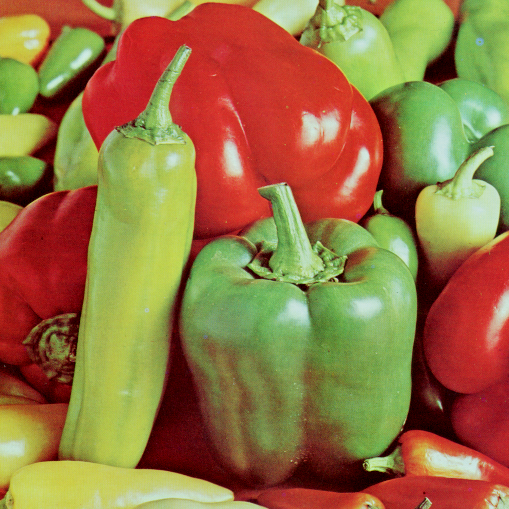
\includegraphics[width=1\textwidth]{peppers-0.png}
    \caption*{$n = 0$ (Original)}
  \end{minipage}
  \hfill
  \begin{minipage}[t]{0.3\textwidth}
    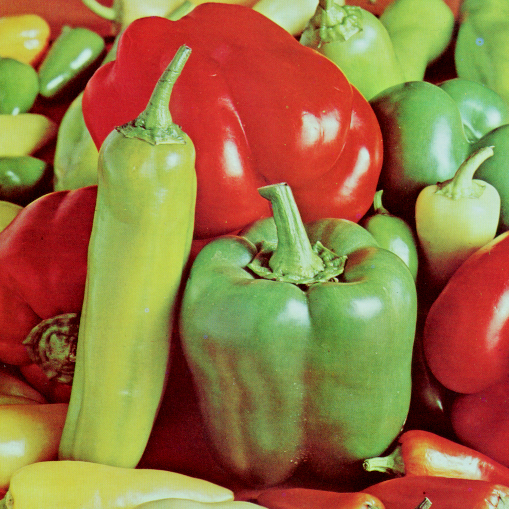
\includegraphics[width=1\textwidth]{peppers-1.png}
    \caption*{$n = 1$}
  \end{minipage}
  \hfill
  \begin{minipage}[t]{0.3\textwidth}
    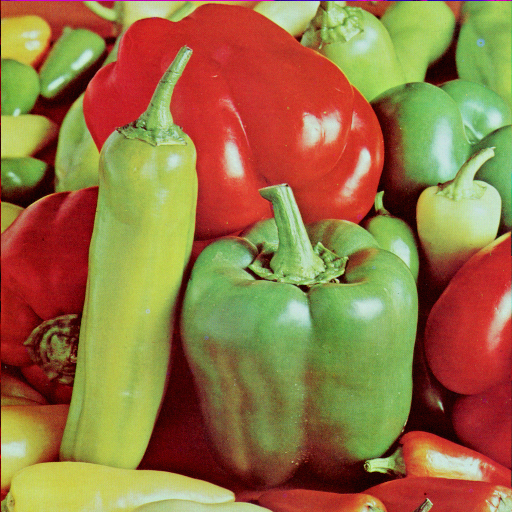
\includegraphics[width=1\textwidth]{peppers-2.png}
    \caption*{$n = 2$}
  \end{minipage}%
  \vspace{0.5cm}
  \begin{minipage}[t]{0.3\textwidth}
    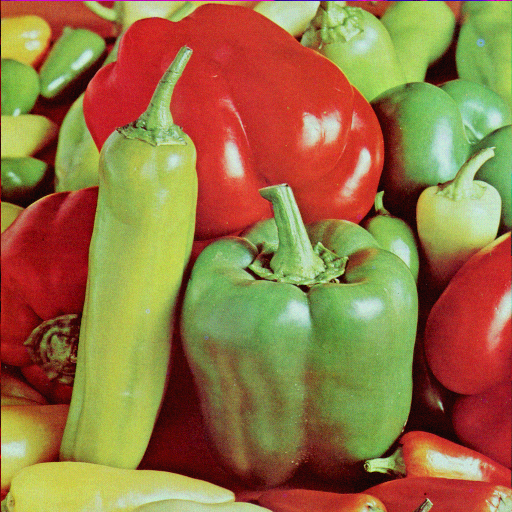
\includegraphics[width=1\textwidth]{peppers-3.png}
    \caption*{$n = 3$}
  \end{minipage}
  \hfill
  \begin{minipage}[t]{0.3\textwidth}
    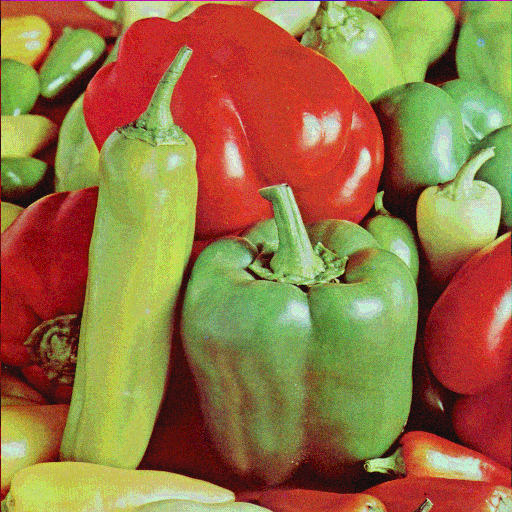
\includegraphics[width=1\textwidth]{peppers-4.png}
    \caption*{$n = 4$}
  \end{minipage}
  \hfill
  \begin{minipage}[t]{0.3\textwidth}
    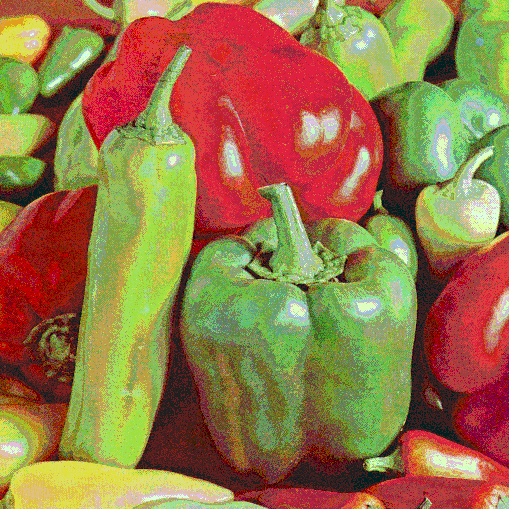
\includegraphics[width=1\textwidth]{peppers-5.png}
    \caption*{$n = 5$}
  \end{minipage}%
  \vspace{0.5cm}
  \begin{minipage}[t]{0.3\textwidth}
    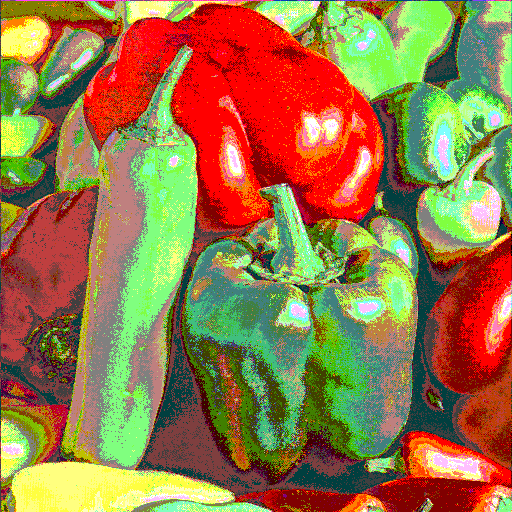
\includegraphics[width=1\textwidth]{peppers-6.png}
    \caption*{$n = 6$}
  \end{minipage}
  \hfill
  \begin{minipage}[t]{0.3\textwidth}
    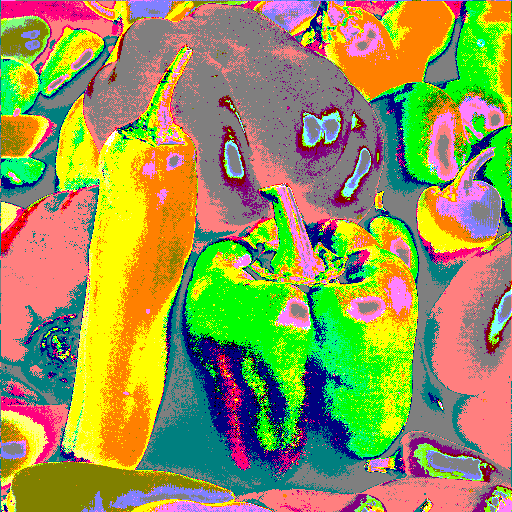
\includegraphics[width=1\textwidth]{peppers-7.png}
    \caption*{$n = 7$}
  \end{minipage}
  \hfill
  \begin{minipage}[t]{0.3\textwidth}
    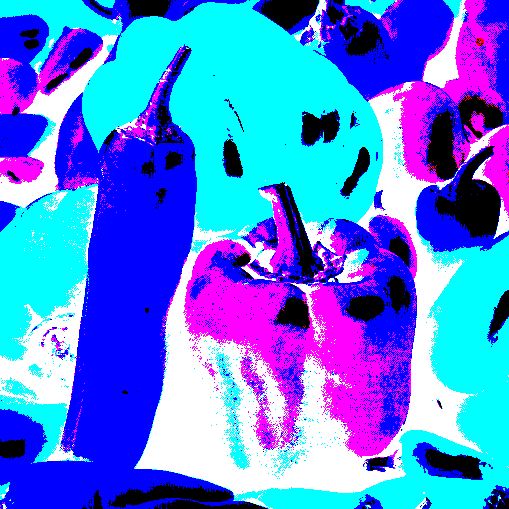
\includegraphics[width=1\textwidth]{peppers-8.png}
    \caption*{$n = 8$}
  \end{minipage}
  \caption{Farbbild Paprika veränderten durch maximalen Fehler für alle $n \in [0,8]$.}
  \label{fig:peppers}
\end{figure}
\noindent
Zusätzlich wird in diesem Beispiel der schlimmste Fall betrachtet.
Das Verstecken einer echten Nachricht wird fast immer
ein besseres Ergebnis liefern, da Nachrichtenbit
zufällig mit den des Bilds überstimmen oder vorherige Fehler
durch weitere Teile der Nachricht wieder ausgeglichen werden.

\section{Beschreibung eines Algorithmus}
Die Möglichkeiten von \acs{lsb}-Verfahren wurden im vorherige Abschnitt gezeigt,
es kann jetzt eine mehr formale Beschreibung gegeben werden,
wie ein solches Verfahren umgesetzt werden kann.
Da ein steganografisches Verfahren die Vertraulichkeit einer Nachricht
nur indirekt sichert, ist es sinnvoll, diese vor dem Verwenden mit einem
als sicher geltenden Algorithmus zu verschlüsseln.

\begin{definition}[\acs{lsb}-Verfahren]
  Es sei $p_{x,y} = (r,g,b)$ ein Pixel und $\mathbf{B} = p^{m \times n}$ ein Bild
  mit $y \in [0, m-1]$ und $x \in [0, n-1]$. Es sei $P$ die Menge aller Pixel von $\mathbf{B}$
  und $f$ eine
  Funktion mit $f: P \setminus \{p_{0,0},p_{m-1,n-1}\} \leftarrow f(\mathbf{B})$.

  \begin{algorithm}
    \DontPrintSemicolon
    \KwIn{image $\mathbf{B}$ and plaintext message $x$}
    \KwOut{image $\mathbf{B}$ with hidden message $y$}
    \Begin(){
      $y \leftarrow e_k(x)$\;
      $n \leftarrow 1$\;
      write message length of $y$ to $p_{0,0}$ and $p_{m-1,n-1}$\;
      \While(){true}{
        \lIf(){$n = 9$}{message is to long}
        $P' \leftarrow f(\mathbf{B})$\;
        \For{$p \in P'$}{
          \For(\tcc*[f]{color values r,g,b}){$c \in p$}{
            $b \leftarrow$ read next bit of $y$\;
            write $b$ at position $n$ of $c$\;
            \lIf(){message done}{\Return{}}
          }
        }
        $n \leftarrow n + 1$\;
      }
    }
    \caption{\acs{lsb}-Verfahren Enkodierung}
  \end{algorithm}
  \begin{algorithm}[H]
    \DontPrintSemicolon
    \KwIn{image $\mathbf{B}$ with hidden message $y$.}
    \KwOut{plaintext message $x$.}
    \Begin(){
      $n \leftarrow 1$\;
      $y \leftarrow \emptyset$\;
      $l \leftarrow$ read message length at $p_{0,0}$ and $p_{m-1,n-1}$\;
      \While(){$l \neq 0$}{
        $P' \leftarrow f(\mathbf{B})$\;
        \For(){$p \in P'$}{
          \For(\tcc*[f]{color values r,g,b}){$c \in p$}{
            $b \leftarrow$ read bit at position $n$ of $c$\;
            $y \leftarrow y \cup \{b\}$\;
            \lIf(){$l = 0$} {
              \GoTo{done}
            }
            \lElse(){$l \leftarrow l - 1$}
          }
        }
        $n \leftarrow n + 1$\;
      }
      \Marker{done}{
        \Return{$d_k(y)$}
      }
    }
    \caption{\acs{lsb}-Verfahren Dekodierung}
  \end{algorithm}
\end{definition}
Damit eine Nachricht im Bild möglichst wenig auffällt, macht es Sinn, Pixel
so auszuwählen, dass diese gleichmäßig verteilt sind. Die Verteilfunktion $f$ hat genau diese
Aufgabe. Das Bild $\mathbf{B}$ wird als Folge der natürlichen Zahlen
$a = 0,1,\ldots,mn - 1$ betrachtet. Durch wiederholtes halbieren von $a$ und
speichern der entstehenden Hälften in einer Warteschlange, kann die Folge nach
dem Prinzip der Breitensuche abgearbeitet werden und es entstehen relativ gleichmäßig
verteile Koordinaten.
\begin{figure}
  \centering
  \begin{minipage}[t]{0.45\textwidth}
    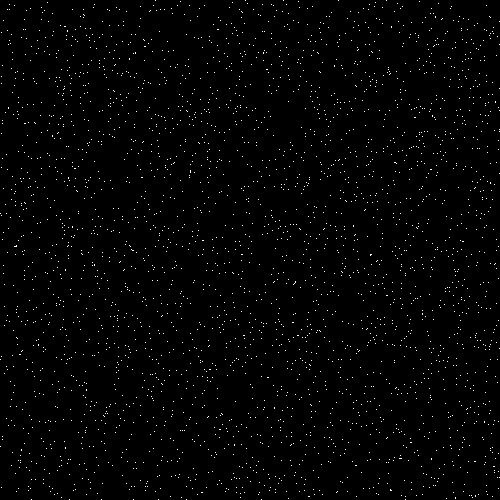
\includegraphics[width=1\textwidth]{black-1200.png}
    \caption*{1200 Byte}
  \end{minipage}
  \hfill
  \begin{minipage}[t]{0.45\textwidth}
    
\includegraphics[width=1\textwidth]{black-3600.png}
    \caption*{3600 Byte}
  \end{minipage}%
  \vspace{0.5cm}
  \begin{minipage}[t]{0.45\textwidth}
    
\includegraphics[width=1\textwidth]{black-10800.png}
    \caption*{10800 Byte}
  \end{minipage}
  \hfill
  \begin{minipage}[t]{0.45\textwidth}
    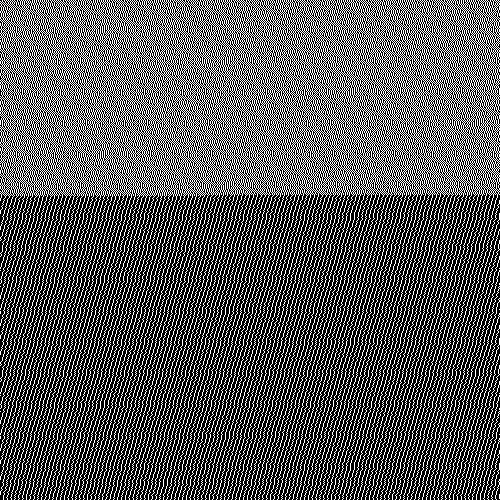
\includegraphics[width=1\textwidth]{black-32400.png}
    \caption*{32400 Byte}
  \end{minipage}
\end{figure}